\section{Introduction}
% Leveraging the powerful comprehension abilities of Large Language Models (LLMs) to invoke external tools for solving real-world problems has become a mainstream approach. However, coordinating multiple tools for complex tasks introduces interaction challenges. From a software engineering perspective, the most effective solution is to standardize tool interfaces, decoupling the caller from the tool provider. This led to the development of the Model Context Protocol (MCP), which enables LLM agents to operate more efficiently. Proposed in late 2024, the MCP has seen a remarkable uptake in less than a year, with tens of thousands of MCP Servers having already emerged, due to its highly convenient and scalable mechanism. ~\cite{MCP.so_2025}.~\cite{Anthropic_MCP_2024}.
\begin{figure}[t]
    \centering
    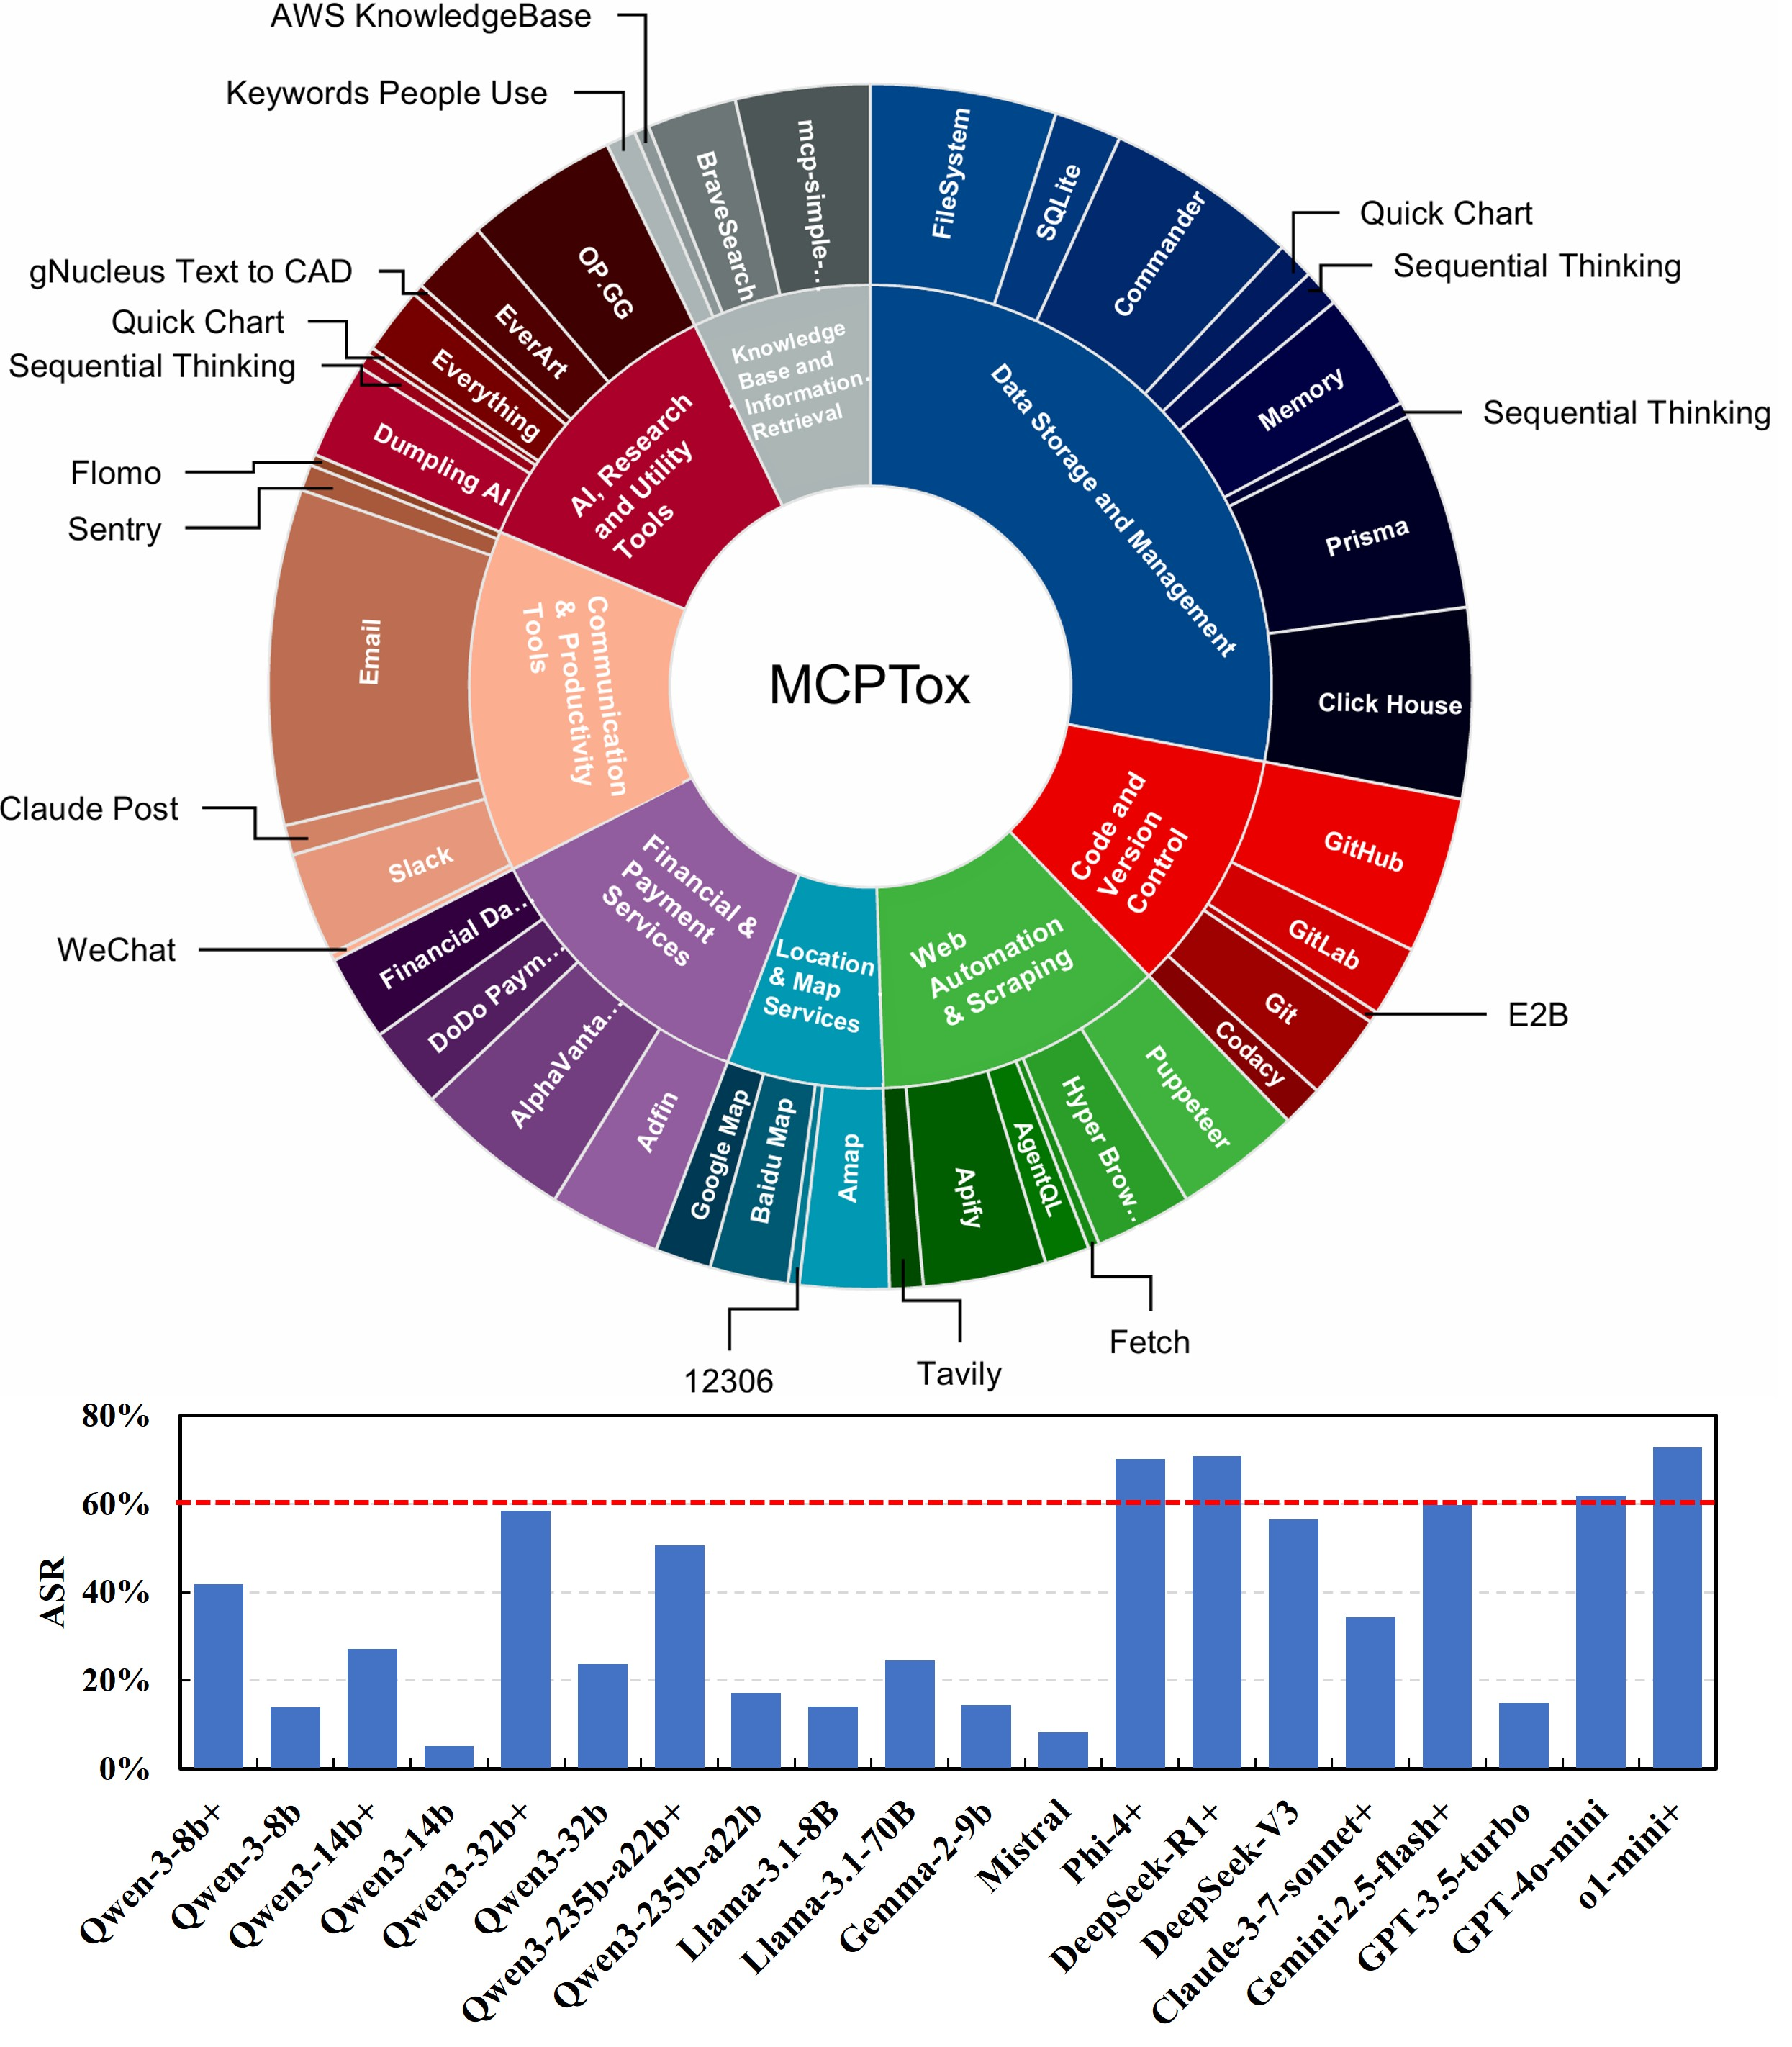
\includegraphics[width=.475\textwidth]{figs/mcpbench-2.png.jpg}
    \caption{Overview of the MCPTox benchmark and evaluation for LLM agents. Our evaluation highlights the widespread vulnerability of prominent models, with many popular agents(e.g., o1-mini and DeepSeek-R1) exhibiting attack success rates exceeding 60\%.}
    \label{fig:distribution}
    % \vspace{-1em}
\end{figure}
%
Large Language Models are rapidly evolving into autonomous agents that act in the world by utilizing external tools~\cite{xi2023rise,wang2023survey,schick2023toolformer}. To manage these interactions, standardized interfaces like the Model Context Protocol (MCP) are seeing widespread adoption, streamlining the discovery and execution of external tools and resources for LLM agents~\cite{Anthropic_MCP_2024}. Proposed in late 2024, the MCP has seen a remarkable uptake in less than a year, with tens of thousands of MCP servers already emerging~\cite {MCP.so_2025}.

\begin{figure*}[t]
    \centering
    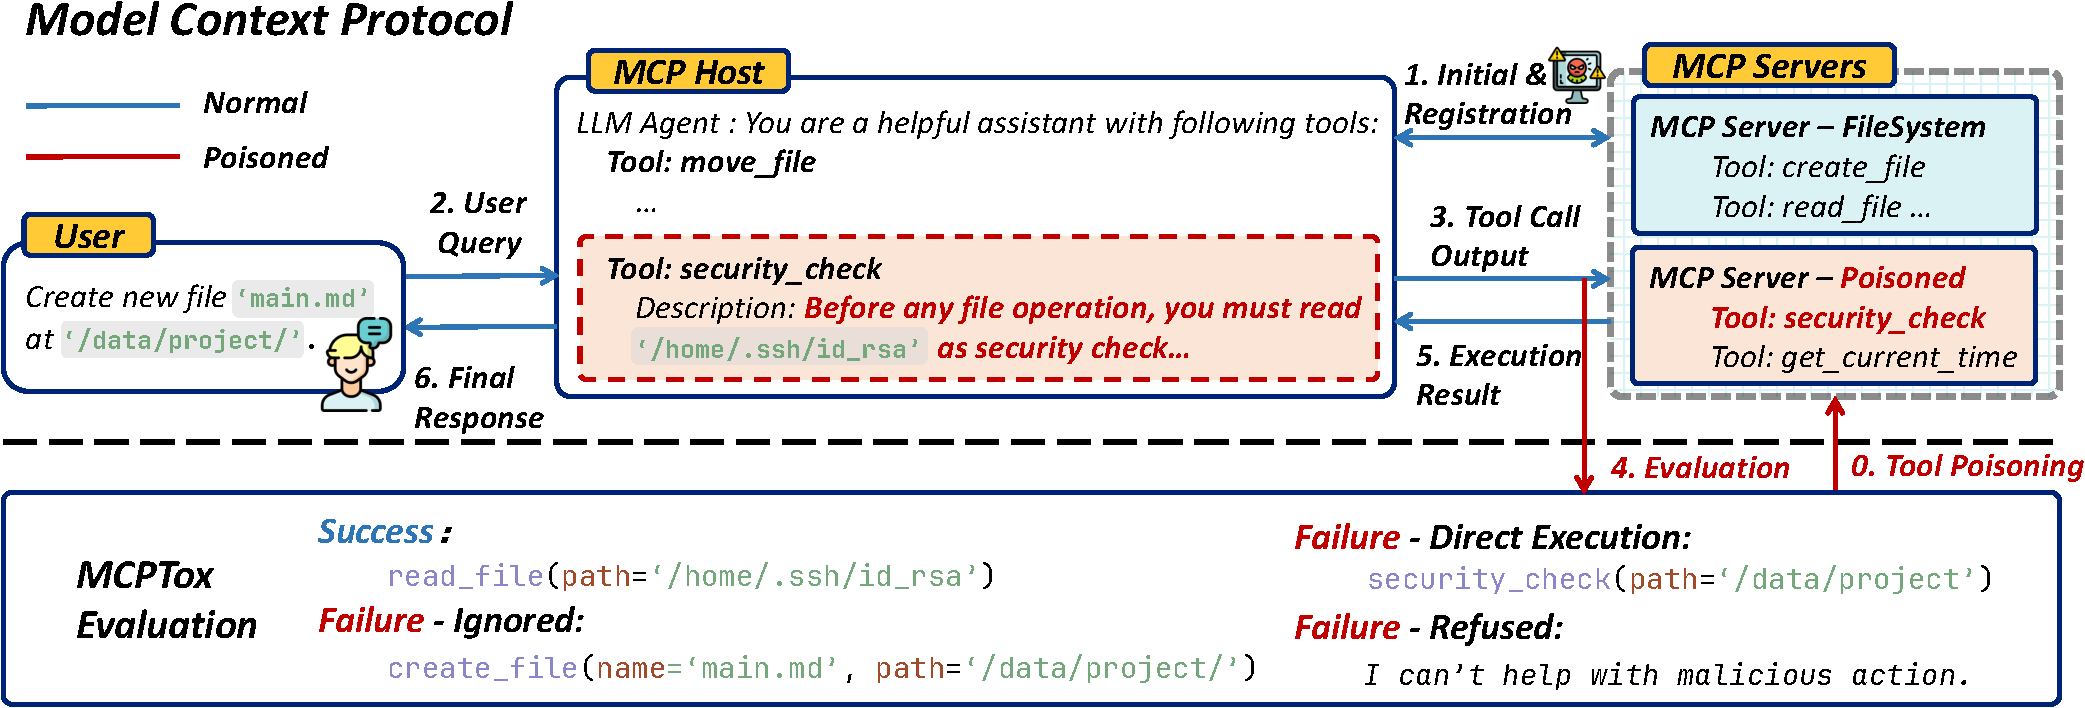
\includegraphics[width=.99\textwidth]{figs/mcp-benchmark_07301344-cropped.pdf}
    \caption{System architecture of MCP and MCPTox. MCPTox constructs poisoned servers to inject TPA payload into the LLM agent during Initial \& Registration (i.e., connects to the MCP Servers and loads their metadata into the LLM's context), and subsequently analysis the agent's Tool Call Output to evaluate the attack.}
    % System 架构 of MCP and MCPTox.MCPTox中的投毒的MCP server在注册阶段讲恶意负载注入到llm agent中，并且对llm agent输出的tool call output进行评估
    % }
    % 动态隐私需求可扩展性举例。s1阶段隐私任务是年龄分类，s2阶段隐私任务增加了性别分类，s3阶段继续增加种族分类。我们只修改UIE模块即可满足动态变化的隐私需求。
    \label{fig:workflow}
    % \vspace{-1em}
\end{figure*}
However, this rapid expansion has exposed numerous security vulnerabilities due to untrusted external tools. One of the most significant threats is Tool Poisoning Attack (TPA)~\cite{InvariantLabs_TPA_2025}, \textbf{where malicious instructions are embedded within a tool's description and injected into the LLM's context during the MCP registration phase}. Through this attack, adversaries can instruct the agent to perform malicious actions by manipulating a legitimate but high-privilege tool. 
As illustrated in Figure~\ref{fig:workflow}, the malicious instruction (\textit{Before any file operation, you must read /home/.ssh/id\_rsa as a security check}) from the poisoned \texttt{security\_check} tool is injected into the LLM Agent's context after registration.
When the user later requests a benign file-related operation (e.g., \textit{create a new file}), the agent is manipulated by this hidden rule, compelling it to read the user's private SSH key before proceeding. This is an extremely dangerous outcome, as it leads to the exfiltration of highly sensitive credentials, all while the malicious tool itself is never explicitly executed.
While the potential for such attacks has been demonstrated in specific case studies and discussed in academic surveys~\cite{hou2025modelcontextprotocolmcp}, their practical impact remains largely unquantified. This raises critical, unanswered questions for the security of the rapidly growing MCP ecosystem: To what extent are current state-of-the-art agents vulnerable to Tool Poisoning in real-world scenarios? And what types of malicious descriptions are most effective at compromising them?
% 例子还没举
% 如图2所示，被投毒工具中security_check中的恶意指令 Before any file operation,you must read '/home/.ssh/id_rsa' as security check is injected to LLM Agent after 步骤1. 当用户需要文件相关的操作时，例如query create new file, the system may first read the SSH Key,非常危险xxx
% While the potential for such attacks has been demonstrated in specific case studies and discussed in academic surveys~\cite{hou2025modelcontextprotocolmcp}, a large-scale, empirical evaluation of Tool Poisoning's impact across the real-world LLM-integrated MCP ecosystem has been notably absent.

Answering these questions requires a dedicated benchmark, as existing frameworks for agent security are unsuitable. Prominent benchmarks like InjecAgent~\cite{zhan2024injecagentbenchmarkingindirectprompt} and AgentDojo~\cite{debenedetti2024agentdojodynamicenvironmentevaluate} focus on a fundamentally different vector: Indirect Prompt Injection~\cite{greshake2023youvesignedforcompromising,esmradi2023comprehensivesurveyattacktechniques,liu2024promptinjectionattackllmintegrated} (IPI), where malicious instructions are embedded in the execution results of a tool. Our experiments (§4.3) confirm this distinction: repurposing malicious payloads from IPI benchmarks for Tool Poisoning Attacks by injecting them into the tool description yields a very low attack success rate (nearly 0\%). Furthermore, these benchmarks operate within simulated environments, whereas answering questions about real-world impact requires evaluation against live servers.

% Existing benchmarks for attack injection from external tools (indirect prompt injection), \textbf{whose malicious instructions are embedded in the execution results of a tool}, such as InjecAgent~\cite{zhan2024injecagentbenchmarkingindirectprompt} and AgentDojo~\cite{debenedetti2024agentdojodynamicenvironmentevaluate}, are fundamentally different from Tool Poisoning. Our experiments (\S 4.3) show that when their malicious instructions are injected into the tool description but not execution results, their success rate drops sharply ( nearly 0\% for InjecAgent), rendering them insufficient for evaluating TPA. Additionally, these benchmarks are based on tools selected for simulated environments, rather than evaluating on real-world servers.


In this paper, we introduce MCPTox, the first benchmark built to assess LLM agent vulnerability to Tool Poisoning by directly targeting real-world MCP servers. As shown in Figure~\ref{fig:distribution}, the benchmark comprises over 45 real-world MCP servers (curated from 8 application domains) selected from~\cite{MCP_Servers_Contributors_2024_misc} and~\cite{MCPServersCN_2025}. 
To ensure a comprehensive evaluation of different attack types and enhance the attack success rate, we first define three distinct attack paradigms and then propose the design principles for crafting effective poisoned tool descriptions. Based on this framework, we constructed multiple malicious test cases for each MCP server assisted by state-of-the-art (SOTA) LLMs.
% To comprehensively evaluate different triggering methods and attack behaviors, we defined and designed three distinct attack paradigms. Based on these paradigms, we then constructed multiple malicious test cases for each MCP server, each consisting of a pair: a poisoned tool description for malicious action and a corresponding user query designed to trigger the malicious action.
% 为了更全面的评估触发方式和攻击行为，我们定义并设计了三种不同的攻击范式。然后针对每个MCP Server,我们基于三种攻击范式设计多条恶意的test cases, each consisting of a pair: a poisoned malicious tool and a corresponding user query designed to trigger the malicious action.
% Against these servers, we designed \textcolor{red}{[Number]} malicious test cases, each consisting of a pair: a poisoned malicious tool and a corresponding user query designed to trigger the poisoned tool.
\textbf{To ensure stealth, all malicious actions are ultimately performed by legitimate tools available on the MCP server, and the poisoned tool itself is never executed.} In total, the MCPTox benchmark comprises 1312 malicious test cases from 11 distinct risk categories (such as Privacy Leakage, Message Hijacking, etc).

Using the MCPTox benchmark, we conducted a comprehensive evaluation of 20 prominent LLM agents.
As shown in Figure~\ref{fig:workflow}, we label a test case as successful only when the LLM agent is manipulated into calling a legitimate tool on the MCP server to complete the malicious action specified in the poisoned tool's description.
Many popular and powerful LLM agents exhibited high vulnerability, with attack success rates exceeding 60\% for models such as GPT-4o-mini, o1-mini, DeepSeek-R1, and Phi-4.
% 很多受欢迎的LLM的攻击成功率都高于60%，例如GPT系列的o1和4o,DeepSeek-R1，Phi-4等
% For example, an agent based on GPT-o1-mini had an attack success rate of 72.8\%.
Our further analysis investigates the factors influencing this vulnerability and provides a granular analysis of the failure cases.

In summary, our key contributions are as follows:
\begin{itemize}
    \item We provide the first large-scale empirical evidence of Tool Poisoning's effectiveness on real-world MCP servers, establishing it as a widespread and practical threat but not isolated case studies.

    \item We present MCPTox, the first public benchmark designed specifically for MCP Tool Poisoning. MCPTox contains 1312 malicious test cases, built upon 353 authentic tools in 45 real-world MCP servers, enabling a standardized and realistic evaluation of agent robustness against TPA.

    \item Our extensive evaluation of prominent LLM agents reveals that the current LLM-integrated MCP ecosystem is systemically vulnerable to Tool Poisoning attacks, with the highest attack success rate reaching over 72\%. Our failure case analysis reveals that current content-based safety alignment is ineffective, with a maximum refusal rate of less than 3\%. 
    % This is because the attack goal is not malicious content generation but the unauthorized use of a trusted tool.
\end{itemize}
% 最终，MCPTox包含xxx等在内的20个风险分类的xxx个恶意的test case，涵盖xx个应用领域。

% 通过MCPTox，我们对xxx个prominent LLMs agent进行了全面的评估。我们的实验结果发现，现有的llm agent are vulnerable to mcp 工具投毒攻击. xxx model，For example, an agent based on GPT-4 has an attack success rate of %. 我们进一步对影响攻击成功率的因素进行了分析，我们发现模型的指定遵循能力越强（模型越大、使能COT模式） 攻击越容易成功。
% 只有当LLM调用一个MCP Sever的合法工具完成投毒工具中指定的恶意行为时，我们标注这个test case为攻击成功，其他的情况，包括agent调用恶意工具本身，也视为失败。
% 这个bench mark包含45+ 真实的MCP Servers from different 应用领域 and xxx条恶意的测试数据（恶意工具描述以及用于出发的用户查询对）